\section{Durchführung}
\label{sec:Durchführung}

Die Durchführung des Versuchs ist in drei Teile Aufgeteilt:
\begin{itemize}
    \item Überprüfung des Bragg'schen Gesetzes
    \item Untersuchung des Emissionsspektrums von Kuper
    \item Untersuchung der Absorptionsspektren verschiedener Materialien
\end{itemize}
Allerdings wird für jeden Teil der gleiche Versuchsapperat verwendet.(siehe \autoref{fig:aufbau})

\begin{figure}
    \centering
    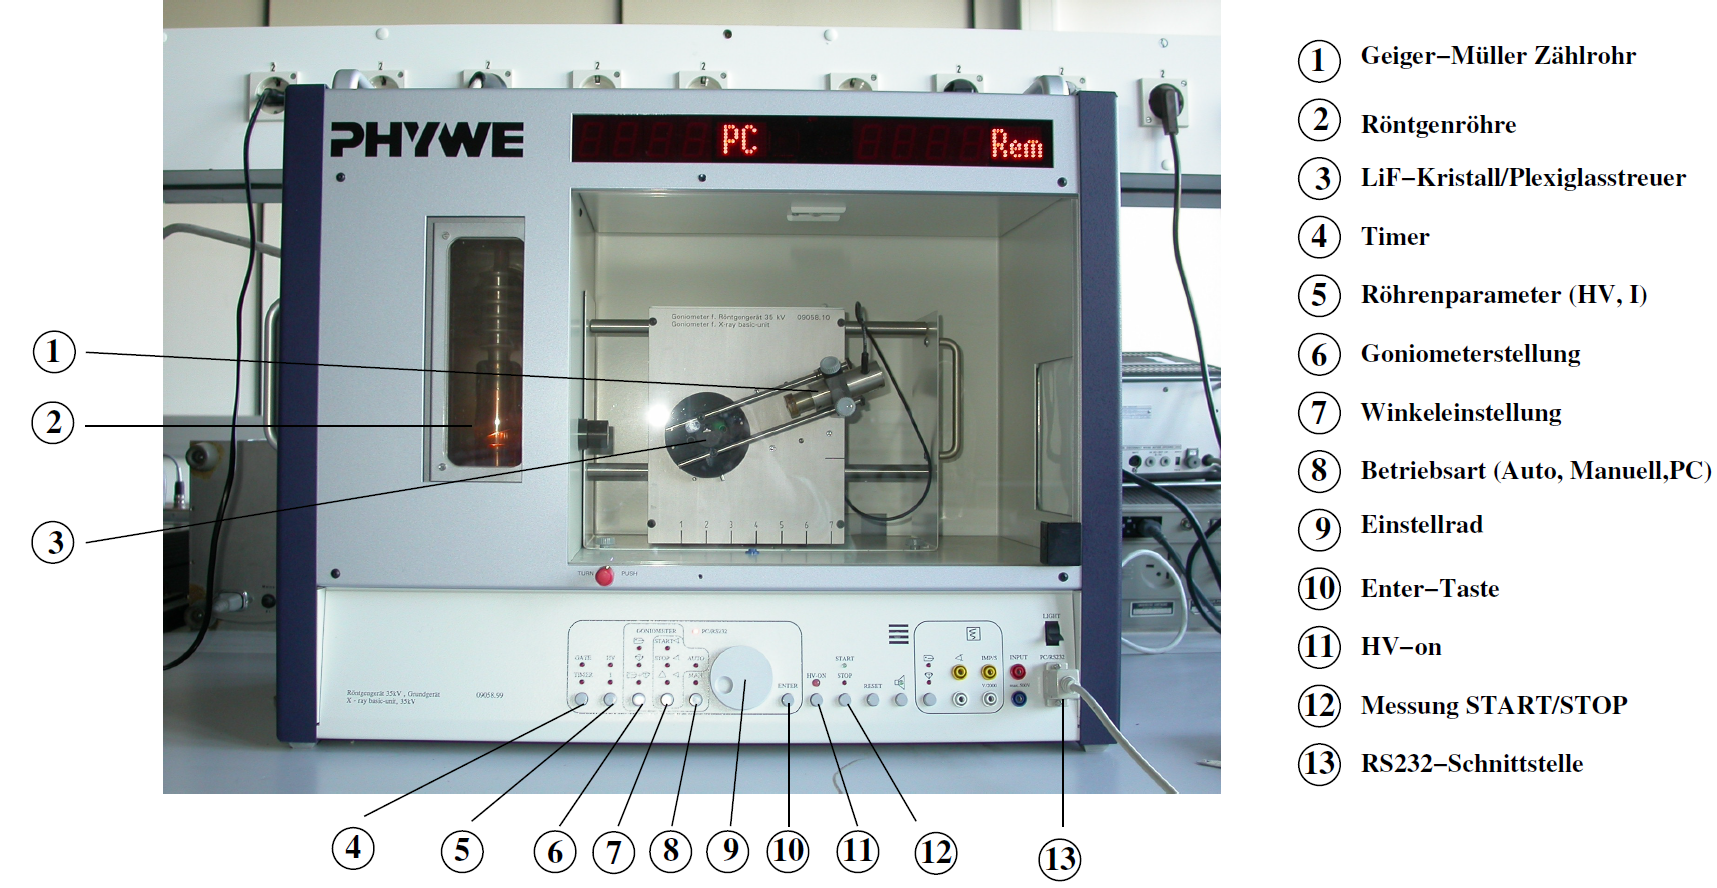
\includegraphics[width=0.8\textwidth]{images/aufbau.png}
    \caption{Versuchsaufbau der Röntgenröhre.}
    \label{fig:aufbau}
\end{figure}

Hier handelt es sich um eine Röntgenröhre, die Strahlung erzeugt, einen LiF-Kristall, an dem die Strahlung gebeugt wird und ein Geiger-Müller Zählrohr welches die Intensität der gebeugten Strahlung misst.
Die Röntgenstrahlung wird mithilfe einer $\SI{1}{\milli\metre}$ Blende (waagerecht zum Boden gedreht) gebündelt und die Winkel des Kristalls und des Geiger-Müller Zählers können variiert werden.
Als Spannung an der Röntgenröhre wird $U=\SI{35}{\kilo\volt}$ und als Strom $I=\SI{1}{\milli\ampere}$ eingestellt.


\subsection{Überprüfung des Bragg'schen Gesetzes}
\label{ssec:bragg}

Um die \autoref{eq:bragg} zu überprüfen wird für den Kristall ein fester Winkel von $\theta=\SI{14}{\degree}$ eingestellt und der Geiger-Müller Zähler läuft von $\alpha=\SIrange{26}{30}{\degree}$ in $\SI{0.1}{\degree}$ Schritten.
Gemessen wird bei einer Integrationszeit von 5 Sekunden.

\subsection{Untersuchung des Emissionsspektrums von Kuper}
\label{ssec:emission}

Um das Emissionsspektrums der Kupfer-Röntgenröhre aufnehmen zu können, muss zuerst der Winkel des Geiger-Müller Zählers an den Winkel des Kristall im Verhältnis 2:1 gekoppelt werden.
Dann wird das Spekrum für den Winkelbereich $\theta=\SIrange{4}{26}{\degree}$ in $\SI{0.2}{\degree}$ Schritten mit einer Integrationszeit von ebenfalls 5 Sekunden gemessen.

\subsection{Untersuchung der Absorptionsspektren verschiedener Materialien}
\label{ssec:absorption}

Um die Absorption untersuchen zu können, muss eine Absorberplatte in den Strahlengang vom LiF-Kristall zum Geiger-Müller Zähler montiert werden.
Nun wird in geeigneter Messbereich in $\SI{0.1}{\degree}$ Schritten und einer Integrationszeit von erneut 5 Sekunden durchlaufen.
Diese Messung wird für die Absorberelemente Zink, Gallium, Brom, Rubidium, Strontium und Zirkonium durchgeführt.